\chapter{Introdução}

Com a crescente ênfase na segurança nacional e global, há uma necessidade crescente e urgente de identificação humana. De acordo com \citeonline{jafri2009survey}, as estratégias tradicionais de reconhecimento de identidade  tais como números PIN\nomenclature{PIN}{Personal Identification Number}, \textit{tokens}, senhas e cartões de identificação tornaram-se obsoletas. Esses métodos de segurança tradicionais estão sendo facilmente fraudados, trazendo preocupações no que diz respeito à sua facilidade de aquisição e utilização por parte de terceiros não-autorizados. Senhas e PINs podem ser esquecidos, roubados ou até mesmo descobertos por pessoas mal intencionadas, e cartões, \textit{tokens}, chaves e similares podem ser perdidos, esquecidos ou clonados \cite{lumini2017overview}. 


De modo a superar essas dificuldades algumas abordagens vêm sendo propostas na literatura visando oferecer identificação automática, precisão e confiabilidade. Dentre essas abordagens destaca-se a biometria que segundo \citeonline{hassaballah2015face} é uma área que abrange uma diversidade de tecnologias utilizadas para fins de identificação pessoal por meio da mensuração e análise dos vários aspectos físicos e comportamentais de cada indivíduo.  As características físicas estão relacionadas com a forma do corpo, incluindo a face, íris, retina, impressão digital, palma da mão, veia do dorso da mão, geometria da mão, lóbulo da orelha, etc. Enquanto as características comportamentais estão relacionadas com o padrão de comportamento de uma pessoa, tais como marcha, assinatura, dinâmica de digitação, voz, etc. De acordo  com \citeonline{filipe2010segmentaccao}, a biometria surge como forma de superar as novas necessidades e desafios, proporcionando maiores níveis de segurança, visto que os traços biológicos não podem ser forjados, furtados, extraviados e esquecidos como ocorre com os métodos de segurança tradicionais.


A biometria vem alcançando muito sucesso por utilizar características físicas e/ou comportamentais de cada indivíduo como método de identificação, de forma que segundo \citeonline{Targino2018_iberamia}, a biometria possui finalidades que buscam aprimorar ou até mesmo suceder os métodos tradicionais de segurança. Segundo \citeonline{jain2004introduction}, a área biométrica está  chegando a tal patamar de segurança por utilizar características que satisfazem quatro requisitos básicos: universalidade – todas as pessoas devem possuir essa característica; distinção – duas pessoas devem possuir características distintas; permanência – a característica deve ser invariante durante um determinado período de tempo; mensurável – é necessário que a característica possa ser medida quantitativamente.




Dentro da biometria temos as modalidades biométricas que são características extraídas do corpo humano, que são únicas para cada indivíduo e que podem ser usadas para estabelecer sua identidade numa população. Dentre as principais modalidades biométricas temos \cite{jain2004introduction}: impressão digital, face \cite{sharif2012survey}, voz, geometria da mão, e padrões de retina e íris \cite{galdi2016multimodal}. De acordo com \citeonline{lumini2017overview,oloyede2017evaluating} a face é a modalidade biométrica mais comumente vista e usada em nossa vida diariamente por ser uma característica universal, única para cada pessoa e possuir boa aceitabilidade em ambientes de captura. Por isso, inúmeros órgãos sejam eles governamentais ou instituições privadas estão mantendo bancos de dados de fotografias de pessoas contendo a face, objetivando identificação do indivíduo. 

Comparada com outras modalidades biométricas tais como impressão digital e íris, a face provê um método de identificação direto, amigável e conveniente \cite{[20]shermina2012recognition}, possuindo várias vantagens como listadas abaixo que a tornam uma das modalidades biométricas mais preferidas para identificação humana:
\begin{itemize}
\item Natureza biológica: A face é uma característica biométrica muito utilizada pelos seres humanos no reconhecimento de pessoas, o que a torna provavelmente a modalidade biométrica mais comum para fins de autenticação e autorização. Por exemplo, no controle de acesso, é fácil para os administradores rastrear e analisar a pessoa autorizada a partir dos dados de face após a autenticação. A ajuda de usuários comuns (por exemplo, administradores) pode melhorar a confiança e a aplicabilidade dos sistemas de reconhecimento, ao passo que os sistemas de reconhecimento de impressões digitais ou de íris requerem um especialista com habilidades profissionais para fornecer confirmação confiável.
\item Não intrusiva: ao contrário de impressões digitais e íris, as imagens podem ser facilmente adquiridas à distância sem contato físico. As pessoas se sentem mais confortáveis para usar a face como identificador em sua vida diária. Um sistema de reconhecimento facial pode coletar dados biométricos de uma maneira fácil, o que é facilmente aceito pelo público.
\item Menos cooperação: em comparação com a íris e a impressão digital, o reconhecimento facial tem uma menor exigência de cooperação entre os sujeitos. Em algumas aplicações particulares, como a vigilância, um sistema de reconhecimento facial pode identificar uma pessoa sem participação ativa dos sujeitos.
\end{itemize}

Atualmente, há progresso significativo em reconhecimento automático de face em condições controladas \cite{min2014efficient}. Entretanto, o desempenho em condições não controladas é ainda insatisfatório  \cite{[4]wei2014dynamic}. Sistemas de reconhecimento facial em ambientes de mundo real, frequentemente, lidam com condições não controladas e não previsíveis tais como grande mudança na iluminação, pose, expressão e oclusão, as quais introduzem variações intraclasse e degradam a performance de reconhecimento. Segundo \citeonline{oloyede2017evaluating,tajima2013performance,min2014efficient} o problema relacionado a oclusão é relativamente pouco estudado na área quando comparado a problemas relacionados a variações de pose, iluminação e expressão. Algumas dessas dificuldades encontradas ao lidar com oclusões em imagens de face em ambientes não controlados podem ser verificadas com o auxílio do trabalho de \citeonline{ghiasi2014occlusion}.




Embora tenha sido dada pouca atenção ao problema de oclusão na literatura de reconhecimento facial, a importância deste problema deve ser enfatizada, pois a presença de oclusão é muito comum em cenários não controlados e pode estar associada a várias questões de segurança. Do ponto de vista do usuário, as oclusões faciais podem ocorrer por várias razões sendo elas intencionais ou não. Em primeiro lugar, acessórios faciais como óculos de sol, cachecol, maquiagem facial, chapéu e boné são bastante comuns na vida diária. Outras pessoas também usam véus por convicções religiosas ou hábitos culturais \cite{min2014efficient}.

Por outro lado, a oclusão também está aparecendo em cenários de segurança e saúde. Por exemplo, a máscara cirúrgica utilizada obrigatoriamente em áreas restritas de hospitais, como também podendo ser frequentemente usada por pessoas na Ásia Oriental (por exemplo, China, Japão) para evitar a exposição a poluição do ar, doenças respiratórias ou alergia ao pólen. Paralelamente nas áreas de construção, existe o capacete de segurança atuando como um instrumento vital, de forma a garantir a segurança das pessoas em tais áreas \cite{du2011hard}.


Dessa forma, identificar as pessoas sem qualquer cooperação de remoção de oclusão devido a acessórios faciais traz grande conveniência e conforto para os usuários em inúmeros cenários. Por outro lado, identificar a presença de oclusões em locais restritos (por exemplo, hospital, área de construção) e revelar a identidade das pessoas nessas áreas garantem a segurança no ambiente. Da mesma forma, a detecção da presença de oclusão pode identificar pessoas suspeitas em certas áreas (por exemplo, estádios de futebol, estações de metrô, caixas eletrônicos, lojas, aeroportos e etc.) e o reconhecimento facial (apesar da presença de oclusão) nessas áreas pode ajudar a polícia a encontrar criminosos/fugitivos. Em outro ângulo  os vândalos e os ladrões de caixas eletrônicos tendem a usar cachecóis e / ou óculos de sol de maneira a impedir que suas faces sejam reconhecidas. Ladrões de bancos e lojas geralmente usam boné ao entrar em lugares em que cometem ações ilegais \cite{[2]zhang2016face}. Na figura \ref{fig:oclusao1} ilustrasse alguns tipos de oclusão, sendo elas oclusões normais e oclusões intencionais.  Em suma, o reconhecimento robusto de face ocluídas parcialmente é muito importante e tem muitos usos potenciais no mundo da vigilância.

\begin{figure}[H]
\centering
\caption{Ilustração de diferentes tipos de oclusões parciais: (a) oclusões faciais comuns em nossa rotina diariamente; (b) oclusões faciais relacionadas a questões de segurança}
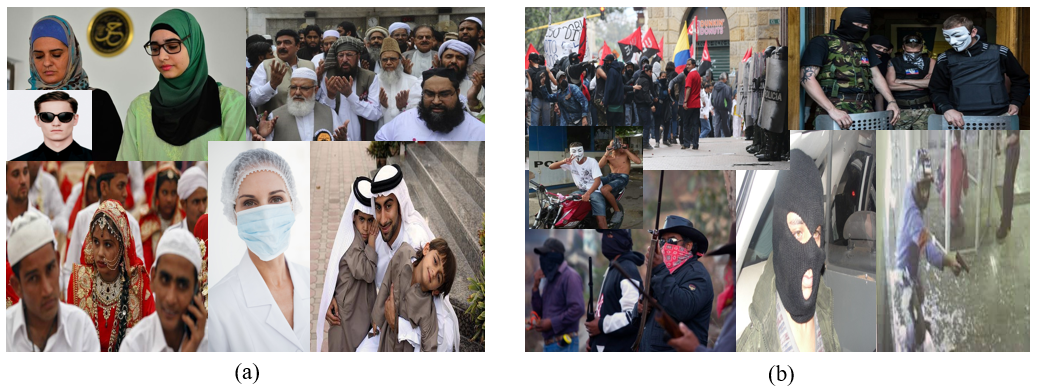
\includegraphics[scale = 0.59]{imgs/varias_oclusoes.png}
\source{Jonas Mendonça Targino, 2018}
\label{fig:oclusao1}
\end{figure}

Nos aplicativos de vigilância, a facilidade de uso é a propriedade mais importante que deve ser considerada, em que nenhuma cooperação do usuário pode ser esperada. Uma ideia intuitiva para atacar oclusões no reconhecimento facial é detectar as regiões ocluídas e então realizar o reconhecimento usando somente as partes não ocluídas. No entanto, os tipos de oclusões são imprevisíveis em cenários práticos e podem impedir a identificação do indivíduo. A localização, tamanho e forma das oclusões são desconhecidas, aumentando assim a dificuldade de segmentação das regiões ocluídas das imagens de face. Segundo \citeonline{min2014efficient} a maioria dos detectores de oclusão são treinados em faces com tipos específicos de oclusões, apresentando mau generalização para vários tipos de oclusões em ambientes reais. 


Tratar com detecção e reconstrução de oclusões parciais em imagens de face não é uma tarefa trivial,  uma vez que a localização, tamanho e forma das oclusões são desconhecidas. Atualmente, a maioria dos detectores de oclusão são treinados em faces com tipos específicos de oclusões apresentando queda de performance quando apresentados aos mais variados tipos de oclusões presentes em ambientes reais. Por exemplo, as variações de pose podem ser reduzidas usando imagens de face com múltiplas vistas de poses ou modelo de face em 3D. Por outro lado, um tipo específico de oclusão (por exemplo, óculos de sol) não pode ser produzida por outros tipos de oclusões (por exemplo, lenço). Logo,  faz-se necessário avaliar o impacto das técnicas de detecção e reconstrução sobre diferentes tipos de oclusão para o reconhecimento biométrico visando identificar os principais prós e contras dessas técnicas como também eventuais limitações.




Existem várias técnicas propostas na literatura para detecção e reconstrução de oclusão em imagens de face. No entanto, não há nenhum estudo que mencione quais técnicas são mais adequadas para determinado tipo de oclusão. Nesse sentido o diferencial dessa pesquisa consiste em realizar um estudo comparativo das técnicas para detecção e reconstrução de faces parcialmente ocluídas, de modo que pretende-se avaliar o impacto dessas técnicas na detecção e reconstrução de diferentes tipos de oclusões em imagens de face visando o reconhecimento biométrico. Como resultado deste estudo, espera-se identificar os principais prós e contras dessas técnicas como também eventuais limitações. 

A presente proposta apresenta um grau significativo de contribuição em termos gerais, abrangendo o estado de arte, suas técnicas, algoritmos para detecção e reconstrução de oclusão e condições de viabilidade de aplicação, levando em conta as variações de iluminação, pose e oclusão. Os resultados obtidos com esta pesquisa serão de grande valia para pesquisadores que estão trabalhando na área, como também iniciantes que almejam conhecimento holístico do estado de arte para desenvolvimento de futuras pesquisas, de modo a produzir um conhecimento e enriquecimento para a área de biometria e para os pesquisadores que tentam colaborar no reconhecimento facial independente das condições de coleta de dados.


\section{Motivação}

Durante a etapa de reconhecimento a existência de oclusões parciais em imagens de face possibilitam queda de performance da estratégia de classificação, visto que existe a ausência de características na imagem da face. Sem contar que o número de trabalhos presentes na literatura que tratam de oclusões parciais quando comparados a outros tipos tipos de variações presentes em ambientes não controlados é relativamente menor. Além dos trabalhos presentes na literatura com fins de detecção e reconstrução de oclusões parciais não explicitarem de maneira clara como o experimento foi realizado, não utilizam uma nomenclatura matemática uniforme e geralmente não disponibilizam o código ou pseudocódigo.

Com isso aumentando a dificuldade de replicação da técnica por outras pessoas ou grupos de pesquisa. Desse modo, torna-se interessante a realização de um estudo comparativo envolvendo técnicas para detecção e reconstrução de oclusões parciais de imagens de face obtidas por meio de bases de dados conhecidas pela comunidade científica e dispostas publicamente, fornecendo com isso um artefato de consulta contendo os prós e contras de cada técnica, seus respectivos códigos, como  também uma notação matemática uniforme.



\section{Objetivos}

O objetivo principal deste trabalho consiste em investigar, implementar e comparar diferentes técnicas para detecção e reconstrução de oclusões parciais em imagens de face humanas visando identificação biométrica em ambientes não controlados com usuários não colaborativos. As técnicas de detecção e reconstrução serão avaliadas em termos da taxa de reconhecimento usando diferentes classificadores (K-vizinhos mais próximos, Máquina de Aprendizado Extremo e Máquinas de Vetores Suporte). Teste de significância estatística será realizado para identificar as melhores e piores técnicas para determinado tipo de oclusão. 
Visando alcançar os objetivos principais, foram adotados os seguintes objetivos secundários:

\begin{itemize}
\item revisão sistemática da literatura buscando encontrar as técnicas para detecção e reconstrução de oclusões parciais em imagens de face presentes na literatura;
\item implementação das principais técnicas de detecção e reconstrução de imagens de face ocluídas;
\item proposição de novas (ou variações) técnicas de detecção e reconstrução de imagens de face ocluídas;
\item emprego das técnicas de detecção e reconstrução de imagens de face ocluídas para reconhecimento biométrico;
\item análise comparativa dos resultados obtidos;
\item publicação dos resultados para que possam ser utilizados pela comunidade científica em trabalhos futuros.
\end{itemize}


\section{Estrutura do documento}
Os capítulos desta dissertação descrevem a teoria necessária para compreensão dos objetivos desta dissertação. Incluindo-se a introdução, os demais capítulos estão organizados da seguinte forma:
\begin{itemize}

\item o Capítulo \ref{cp:cap2}  apresenta uma fundamentação teórica sobre biometria, sistemas biométricos e tipos de ambientes de coleta de dados que servirão como base para o entendimento do corpo dessa dissertação;

\item  no Capítulo \ref{cp:3_rec_facial} são abordados alguns conceitos fundamentais sobre a modalidade biométrica de face, seus prós e contras, tipos de ambientes e técnicas de detecção da região facial.

\item o Capítulo \ref{cp:5_reconstrução} detalha as técnicas presentes na literatura  para detecção e reconstrução de oclusões parciais em imagens de face que foram implementadas neste trabalho.

\item enquanto no Capítulo \ref{cp:6_extracao} são apresentadas as técnicas para extração das características e classificação utilizadas nesse trabalho;

\item o Capítulo \ref{cp:7_proposta} aborda  a proposta de pesquisa, como também seus objetivos. Além de apresentar as três técnicas para reconstrução de faces criadas durante o desenvolvimento deste estudo comparativo;

\item apresenta-se no Capítulo \ref{cp:8_Res_exp} uma breve descrição dos experimentos preliminares, bases de dados utilizadas, formas de pré-processamento das imagens, estratégias de extração das características, configurações dos experimentos e os resultados.

\item no Capítulo \ref{cp:9_Considerações Finais} são apresentados os comentários conclusivos deste trabalho, como também perspectivas futuras;

\item no Apêndice \ref{apen2:RS} é apresentado o método de elaboração da Revisão Sistemática (RS) efetuada juntamente com este trabalho;
\item no Apêndice \ref{apen3:conducao_Revisao} é exposta a estratégia de condução dos artigos advindos da RS;
\item paralelamente no Apêndice \ref{apen4:contextualizacao_literatura} é realizada uma breve contextualização da literatura de técnicas para detecção e reconstrução de oclusões parciais em imagens de face visando o reconhecimento biométrico;
\item enquanto no Apêndice \ref{apen6:matrizes_confusao} são apresentadas todas as matrizes de confusão de cada técnica de reconstrução sobre os quatro grupos de oclusões naturais da base AR.

\item por último e não menos importante no Apêndice \ref{apen7:resultados} são apresentadas todas as tabelas de resultados de acurácia de cada técnica por classificador e nível de decomposição utilizado. Dessa forma possibilitando eventuais consultas conforme a necessidade.

\end{itemize}
